\documentclass[12pt]{article}

\usepackage[spanish]{babel}
\usepackage[utf8]{inputenc}
\usepackage{graphicx}
\usepackage{geometry}
\usepackage{xcolor}
\usepackage{fancyhdr}
\usepackage{lastpage}
\usepackage{pdfpages}
\usepackage{listings}

\geometry{top=25mm,left=15mm,right=15mm,a4paper}

\pagestyle{fancy}
\fancyhf{}
\lhead{Sistemas Operativos}
\cfoot{Página \thepage\ de \pageref{LastPage}}

\graphicspath{./}

\begin{document}
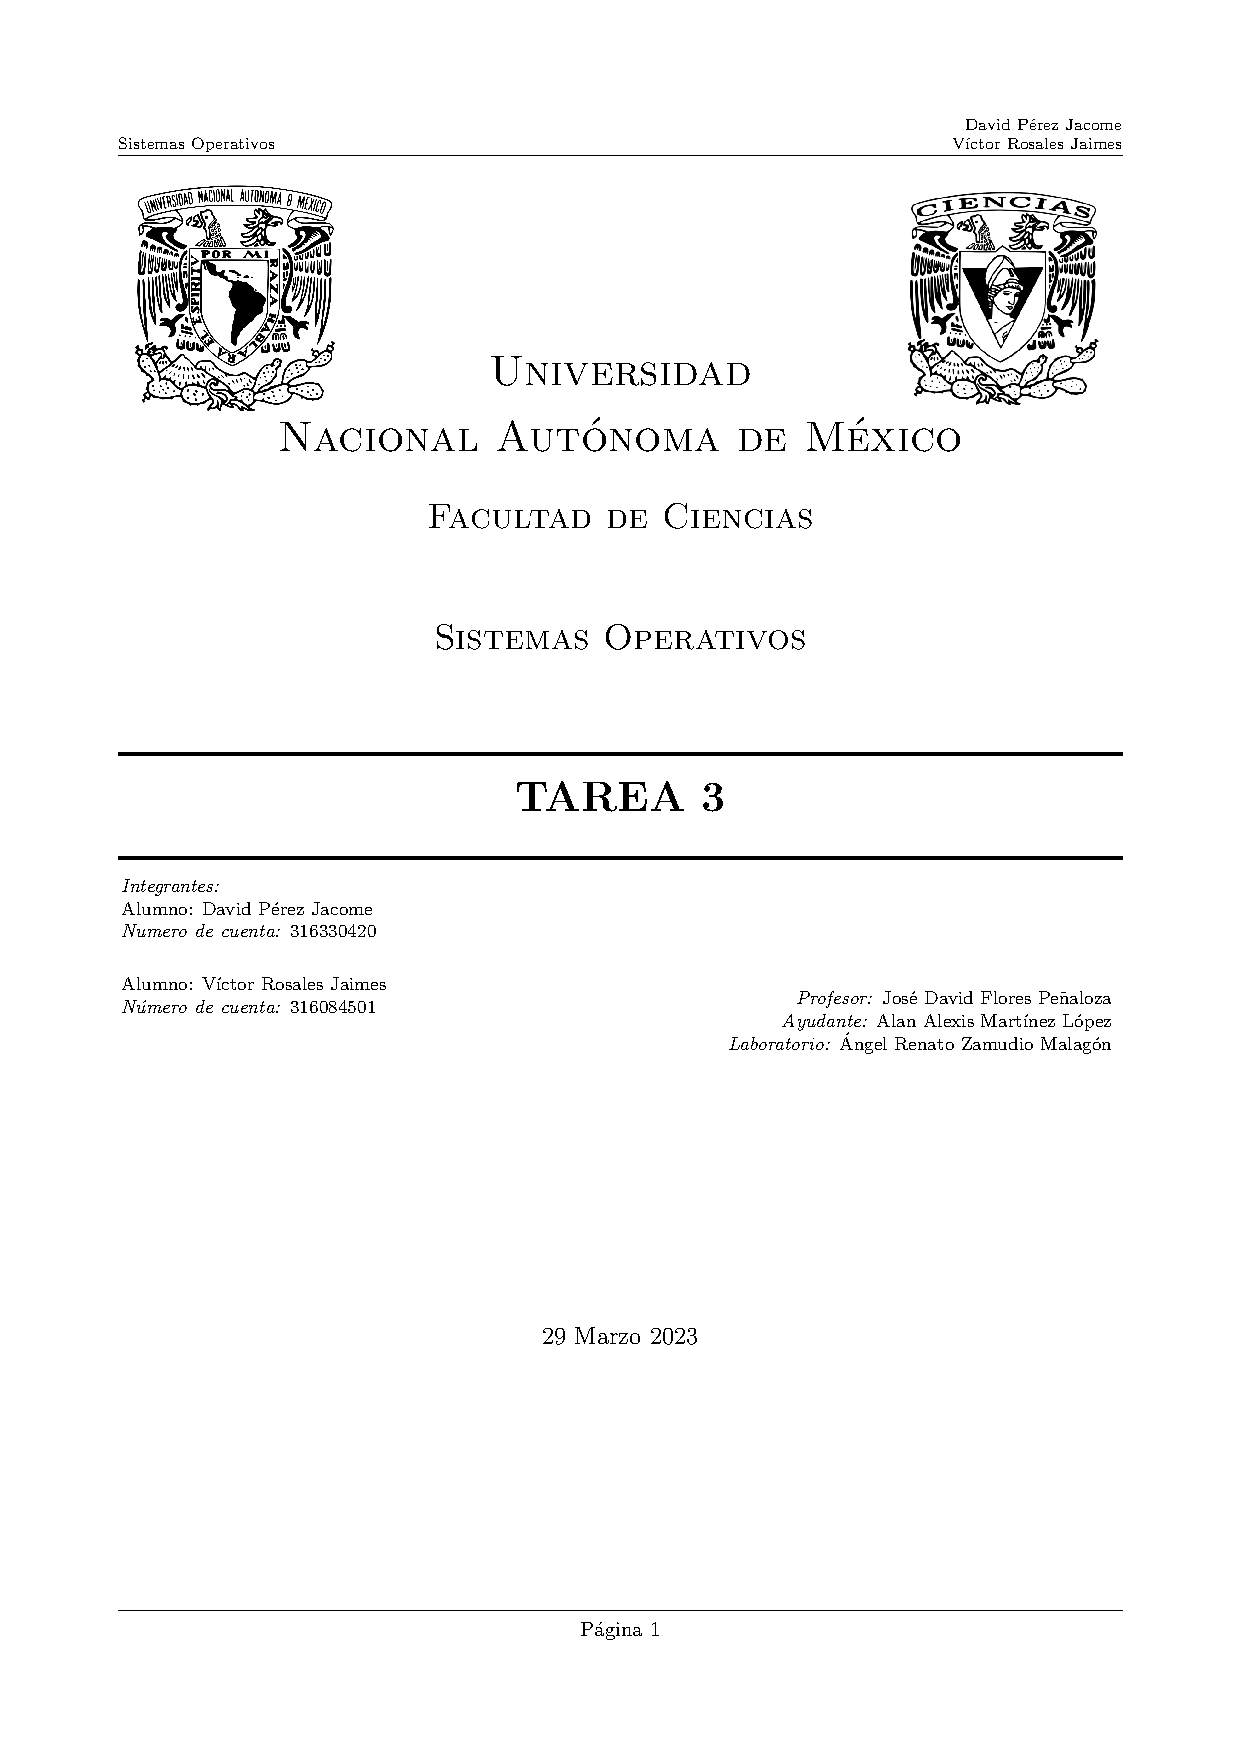
\includepdf{Portada.pdf}
{\color{blue} \section*{Tarea 3.}}

{\color{blue} \subsection*{Instrucciones.}}
\vspace{0.5em} 

Lee con atención las preguntas y contesta lo correspondiente. La tarea se entregará por vía classroom
en un archivo pdf que debe tener el nombre completo y número de tarea, ya sea en una portada o en el encabezado.
\textbf{La tarea se entregará de manera individual.}\\

{\color{blue} \subsection*{Ejercicios}}
\vspace{0.5em}

\begin{enumerate}
    \item Menciona y describe las 3 formas de pasar los parametros a una llamada al sistema.
    \vspace{2mm}

    \textbf{Las 3 formas de pasar parametros a una llmada al sistema son:
    \begin{enumerate}
        \item Pasar los parametros en registros: Se pasan mediante registros de la CPU que al ser rapidos
        de acceder es un tanto eficiente aunque los registros se limitan a 8 registros.
        \item Pasar los parametros en la pila: Se pasan mediante la pila del programa, puede manejar cualquier cantidad de parametros pero
        es un tanto más lenta dado la sobrecarga de acceder a la pila.
        \item Pasar los parametros en un bloque de memoria: Este bloque se asigna en el espacio de direcciones del proceso que llama al sistema, 
        despúes la llamada recibe esta dirección y extrae los parametros, permite el manejo de cualquier cantidad de parametros y es más rapida que
        la pila.
    \end{enumerate}}

    \item ¿Qué elementos debe contener un Boque de control de procesos(BCP)?
    \vspace{2mm}
    
    \textbf{El bloque de control de proceso es una tabla que administra las caracteristicas de un proceso y principalmente debe de tener: 
    \begin{enumerate}
        \item Estado del proceso.
        \item Contador del programa.
        \item Registros del CPU.
        \item Información sobre el calendarizador-CPU.
        \item Información sobre el gestor de memoria.
        \item Información relacionada con el CPU (tiempo de uso, limites de tiempo, etc.).
        \item Información de E/S
    \end{enumerate}}
    
    \item ¿Qué es el descriptor de hardware del proceso?
    \vspace{2mm}

    \textbf{Es otra manera de llamarle al Bloque de Control de Proceso, simplemente es una estructura de datos para la gestión de los procesos, permite manejarlos, tener control y que sean visibles para el sistema operativo.}

    \item ¿Por qué es necesario que exista un descriptor de hardware del proceso?
    \vspace{2mm}

    \textbf{Justamente para que el Sistema Operativo pueda tener control sobre los procesos, por ejemplo cuando el sistema operativo cambia de un proceso a otro se usa para
    guardar el estado actual del proceso en ejecución (cambio de contexto) y esta estructura de datos le perimite gestionar y acceder a los procesos.}

    \item Si tenemos un BCP por cada proceso ¿Cómo tenemos control de todos ellos?
    \vspace{2mm}

    \textbf{Tenemos control sobre los procesos o más bien sobre cada  PCB mediante algoritmos de calendarización que se encargan de controlar los procesos, además de la actualización de los campos del PCB.}

    \item ¿Qué es, como se le dice y cuáles son las caracteristicas y tareas del manejador de interrupciones de primer nivel?
    \vspace{2mm}

    \textbf{Se le conoce como "First-Level Interrupt Handler" (FLIH) y es el responsable de responder adecuadamete a las señales procedentes tanto del exterior de la CPU (interrupciones de un controlador)
    como de dentro del procesador (excepciones y llamadas al sistema), tiene 2 tareas principalmente:
    \begin{enumerate}
        \item Determinar la fuente u origen de la interrupción.
        \item Para iniciar el servicio de la interrupción. 
    \end{enumerate}Todo este proceso lo hace, despues de identificar la fuente de la interrupción, identifica el proceso que se estaba ejecutando (consulta PCB), despues de ello maneja la
    interrupciónya sea activar un dispositivo o realizar operaciones de E/S, despues del manejo de interrupciones restaura el proceso que se estaba ejecutando para que continue con su
    ejecución.}
    \item ¿Cómo se determina de donde viene una interrupción?  
    \vspace{2mm}

    \textbf{Mediante el controlador de interrupciones o rutina de servicio de interrupción el cual simplemente se encarga de determinar su origen y responder a ella de manera adecuada.}

    \item ¿Qué es y que hace una Skip chain?
    \vspace{2mm}

    \textbf{Es una estructura de datos que se utiliza en sistemas operativos para implementar colas de procesos o de threads (lista enlazada con "saltos") y principalmente la usamos para poder ordenar
    los procesos o threads por algún criterio como su prioridad.}
    
    \item Explica cuáles son las tareas del despachador.
    \vspace{2mm}

    \textbf{El despachador simplemente lo que hace es:
    \begin{enumerate}
        \item Seleccionar el proximo proceso a ser ejecutado: dado ya sea su prioridad, o disponibilidad de recursos el despachador selecciona el siguiente proceso que use el procesador.
        \item Cambiar el contexto de ejecución: debe de cambiar  la información en los registros del procesador para que coincidan con los del proceso o thread seleccionado.
        \item Asignar recursos: Debe asegurarse de que el proceso o thread seleccionado tenga acceso a los recursos que necesita para su ejecución.
        \item Control de la ejecución: Debe monitorear su comportamiento, ya sea que use mucho CPU este puede interrumpir su ejecución.
    \end{enumerate}}

    \item Explica cuáles son las tareas del calendarizador.
    \vspace{2mm}
    
    \textbf{Simplemente:
    \begin{enumerate}
        \item Debe saber como asignar el tiempo de CPU entre los procesos o threads que estan en espera en este caso dada su prioridad.
        \item Debe de monitorear la ejecución de los procesos y threads y ver si es necesario interrumpir la ejecución de este para dejar a otro.
        \item Debe de manejar las prioridades para que los de mayor prioridad tengan acceso antes al CPU que los de menor prioridad.
        \item Debe de evitar la hambruna mediante envejecimiento de tareas en los procesos de espera
    \end{enumerate}.}

    \item ¿Qué es la concurrencia real y concurrencia aparente? 
    \vspace{0mm}
    \textbf{\begin{enumerate}
        \item Concurrencia Real: Cada proceso se ejecuta en un solo procesador.
        \item Concurrencia Aparente: Concurrencia emulada ya que se corren varios hilos en un procesador.
    \end{enumerate}}

    \item ¿Qué es el no-determinismo?
    \vspace{2mm}
    
    \textbf{Es cuando no es posible que podamos saber con certeza que es lo que va a pasar, que no podamos predecir con certeza el resultado de una acción.}

    \item ¿Qué es un programa o rutina?
    \vspace{2mm}
    
    \textbf{Especificación de uno o varios procesos (definición concurrente). Conjunto de instruccione sy datos qued escriben los pasos de una tarea.}

    \item ¿Qué es un procesador y cuál es su función?
    \vspace{2mm}
    
    \textbf{Es un agente que ejecuta las instrucciones de u programa para llevar a cabo un proceso.}

    \item ¿Qué es un semáforo y para qué sirve?
    \vspace{2mm}
    
    \textbf{Una variable entera positiva (tipo de dato abstracto) definido por sus metodos wait(s) y signal(s).}

    \item Explica con tus palabras que es Exclusión Mutua.
    \vspace{2mm}
    
    \textbf{Si tenemos 2 procesos A y B, entonces solo uno de ellos puede entrar a su sección critica a la vez.}

    \item Explica con tus palabras que es Deadlock (interbloqueo).
    \vspace{2mm}
    
    \textbf{Los procesos se quedan esperando un estado que nunca va a suceder.}

    \item Explica con tus palabras que es Hambruna.
    \vspace{2mm}
    
    \textbf{Cuando un proceso nunca tuvo tiempo de uso de procesador.}

    \item Explica con tus palabras que es Sección Critica.
    \vspace{2mm}
    
    \textbf{Es la parte del codigo donde se encuentran y se modifican los recursos compartidos.}

    \item Explica con tus palabras que son las condiciones de competencia.
    \vspace{2mm}
    
    \textbf{Es cuando dos procesos acceden a un recurso compartido sin control y modifican este dependiendo de cual llegue primero y esto puede ocacionar inconsistencia o errores en los datos.}

    \item Explica con tus palabras que es la sincronización en cuánto a concurrencia.
    \vspace{2mm}
    
    \textbf{Protocolo para el intercambio de forma ordenada (P1 avisa a P2 que acabo de usar el recurso compartido).}

    \item ¿Por qué la implementación de \textbf{wait} tiene que tener acceso directo al despachador de procesos?
    \vspace{2mm}

    \textbf{Porque wait() al decrementar el semaforo este se bloquea y para desbloquearlo se necesita que otro proceso haga el signal y en el despachador hacemos este cambio de procesos.}

\end{enumerate}

\end{document}